\section{Implementation}
\label{sec:implementation}
We implemented a prototype of the \thename design using a cycle-accurate full system simulation~\cite{gem5}. Regarding the low-level simulation configurations,  we referenced well-documented industry-grade products~\cite{upmem} and simulation configurations from other works on PIM ~\cite{smcsim,obfusmem,ambit,tesseract}. Our simulation is well modularized and generalizable; the hardware components that we implement can be easily modified and provides well-defined APIs for writing host-side and PIM-side applications. 

%In our simulation, the PIM cores are modeled as general-purpose processing cores.

\begin{figure}[h]
    \centering
    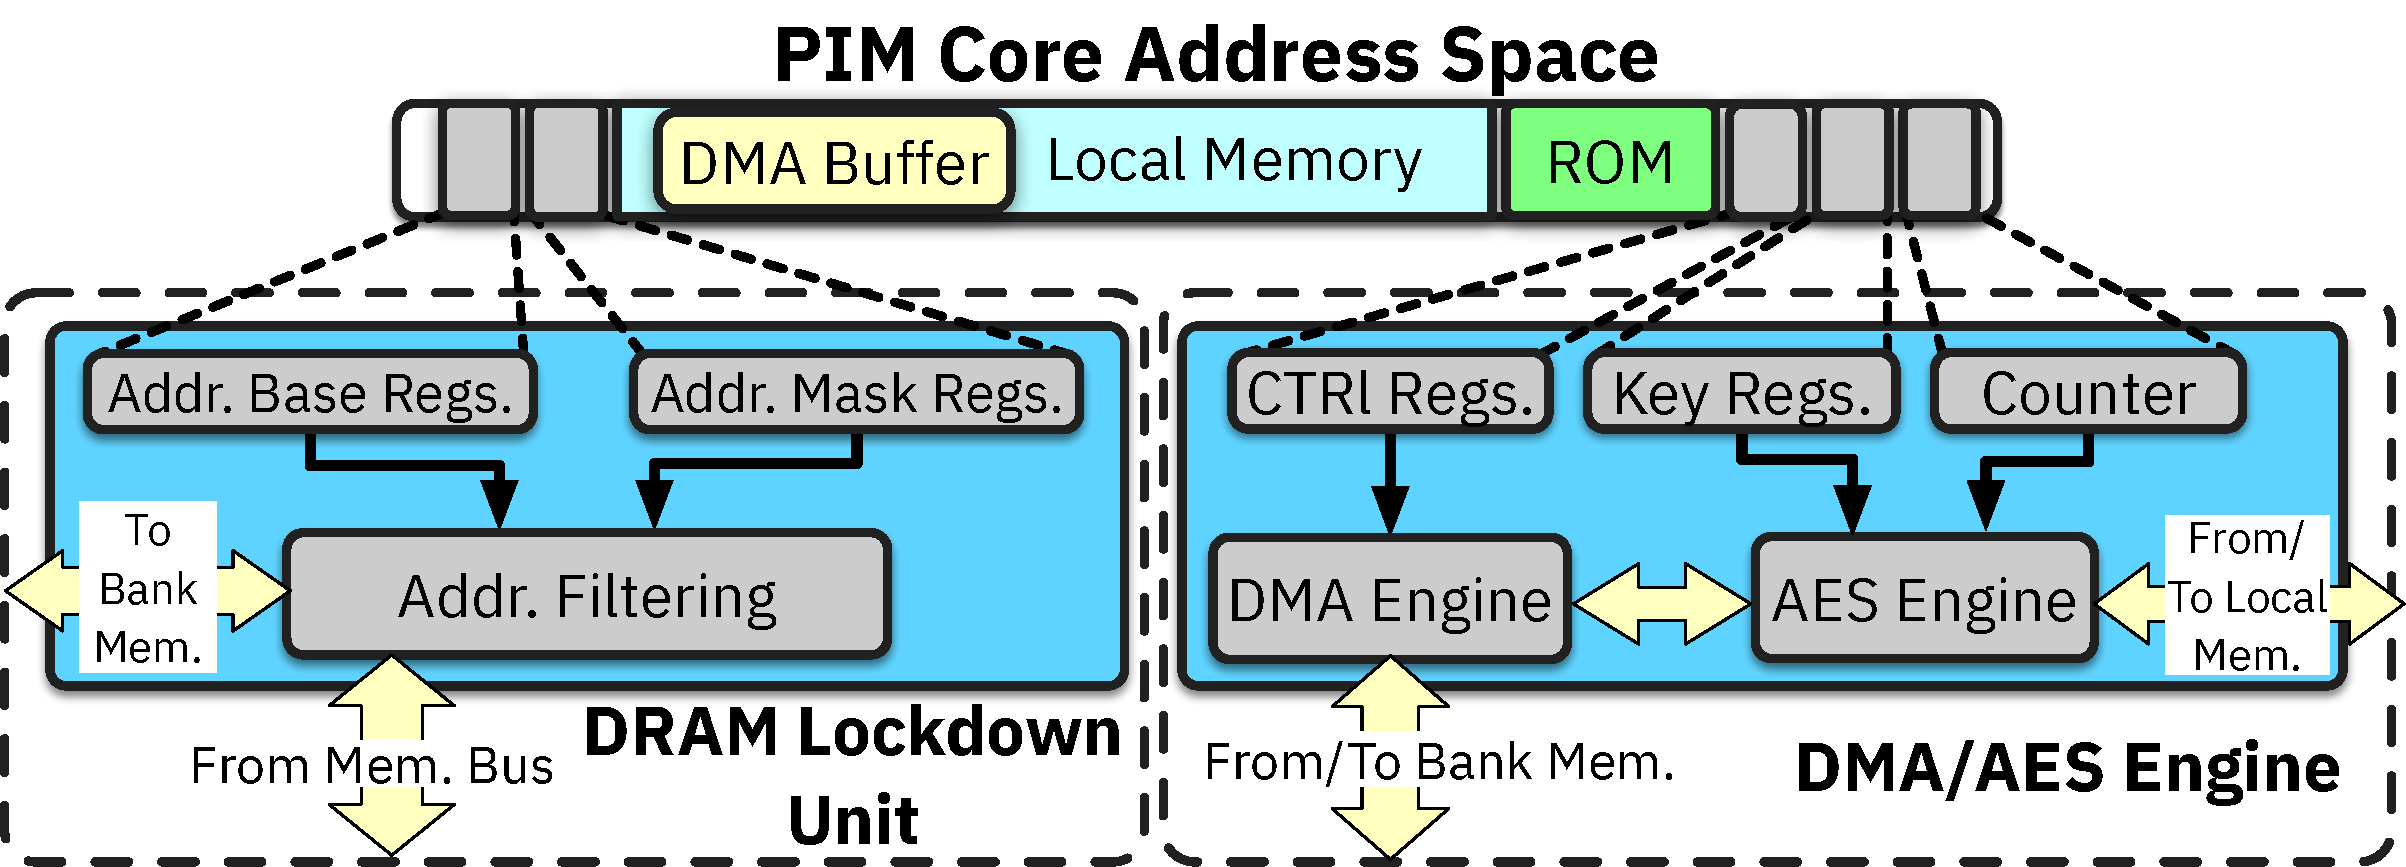
\includegraphics[width=.8\textwidth]{figures/sepim/implementation.pdf}
    \caption{The address space of a PIM core. The control registers of the DRAM lockdown unit and the AES-enabled DMA engine is mapped into the address space of the PIM core for MMIO communication.}
    \label{fig:access-control-dram}
\end{figure}

% \hdr{Simulating PIM systems. } Each PIM core is implemented as a separated simulation system.

% gem5 allows for multiple systems to be simulated simultaneously. This allows us to implement each PIM system as a separated system, and connect them to the host using

% The DMA channel is configured upon device initialization by the host enclave writing the address and size of the DMA region into the registers of the PIM core. The configuration step is necessary because since we disallow the host to access PIM local memory directly (\cref{subsec:memory}), there is no other method to set up the DMA channel for parameters of commands. The content passed through this channel is encrypted with the session key shared after the key exchange using AES-GCM with a counter to prevent replay attacks. The PIM core retrieves the parameters the same way it fetches encrypted batch of data into local memory, using the AES-enabled DMA engine (\cref{subsec:performance}). The exact mechanism for parameter transfer is also applied.

% \subsection{Read-only Memory}
% We implement the Read-only memory, which contains several methods for key exchange and attestation inside 

%\subsection{\thename Core Address Space}


\begin{table*}[t]
    \centering
    \begin{threeparttable}
    \footnotesize
	\renewcommand{\arraystretch}{0.9}
	\renewcommand{\theadgape}{\Gape[.2pt]}
  	\renewcommand\theadfont{\bfseries}
    \begin{tabular}{p{2.5cm}p{3.2cm}p{3.5cm}p{4cm}}
        \toprule
        \thead{Command}&\thead{Parameters}&\thead{Results}&\thead{Description}\\
        \midrule
        \texttt{GET\_CERT\textsuperscript{\dag}}              & - & \texttt{PIM\_CERT} &         Get \thename's certificate\\ 
        \texttt{SET\_SESSION\_KEY}      & \texttt{SESSION\_KEY} & - & Send encrypted session key to PIM\\ 
        \texttt{SET\_DATA\_KEY}         & \texttt{DATA\_KEY} & - & Send data decryption key to PIM\\ 
        \texttt{LOAD\_KERNEL}           & \texttt{KERNEL\_BINARIES} & \texttt{LOCAL\_MEM\_MEASUREMENT}&         Load PIM kernel\\
        \texttt{EXECUTE}\textsuperscript{*}                & \texttt{FN\_NAME, FN\_ARGS} & \texttt{RESULTS} &         Command PIM to execute the kernel\\ 
        \texttt{LOCK\_MEM}              & - & \texttt{BANK\_MEASUREMENT} &         Enable DRAM lockdown\\
        \texttt{MEMCPY}                 & \texttt{DST\_ADDR, SRC\_ADDR, SZ} & - &         Move data within the memory bank during lockdown mode\\        
        \texttt{ACCESS\_DATA}           &\texttt{DATA, ADDR, SZ, OP}& \texttt{DATA} &         Data access during lockdown mode\\        
        \texttt{UNLOCK\_MEM}            & - & - & Disable DRAM lockdown\\
        
        \texttt{DESTROY}\textsuperscript{\dag}                & - & - &         Stop \thename execution, clear local memory and unlock bank\\
        \bottomrule
    \end{tabular}
    
	\begin{tablenotes}
	    \item \hfil \textsuperscript{*} parameters and results are defined by \thename kernel; \textsuperscript{\dag} does not require authentication.
	  %  \textsuperscript{*} data is contained on user's device;
% 			\item \hfil\textsuperscript{\dag};
% 			\textsuperscript{*}
		\end{tablenotes}    
    \end{threeparttable}
    
    \caption{Commands supported by \thename, their parameters, results, and descriptions.}
    \label{tab:commands}
\end{table*}


\subsection{PIM Core and ROM}
We implement the PIM cores as general-purpose execution cores that use the local memory as their RAM and have low-latency access to the memory banks. The specifications for the cores are described in~\autoref{table:config}. \autoref{fig:access-control-dram} demonstrates the address space of the PIM core and the memory mapping of the components into the address space. Local memory is mapped into the address space of \thename as a contiguous memory region, which it uses as the memory for its code (the \thename kernel), the stack space, and DMA transfers. The PIM core communicates with other hardware components using MMIO. The registers of the AES-enabled DMA engine and the DRAM lockdown unit are memory-mapped to fixed addresses so that the PIM core can configure and send commands to the components.

ROM contains the code for cryptographic primitives (e.g., key generation) and functions for handling the commands. The list of supported commands is demonstrated in \autoref{tab:commands}. Our prototype implements ROM code directly inside the PIM kernel code and loads it to the local memory. This would simplify the implementation while achieving the same functionality and performance characteristics. ROM must be implemented in a separated read-only memory module to protect the security-sensitive code against tampering in an actual implementation. Moreover, PIM core should be implemented so that only the attestation code can access the key storage containing the root endorsement key to prevent key leakage. As noted by \cite{minimalist}, the requirement can be easily enforced with an introduction of a hardware monitor on a PIM core's program counter that only allows access to the EK when the PC is within the attestation code.

%Finally, it is crucial to prevent a malicious enclave from leaking the EK. First, we only allow the attestation procedure to access the EK.  Moreover, for each newly created \pimenclave, a new public and private key pair used for attestation is derived from the EK to prevent information leakage. 
% \subsection{ROM}

\subsection{AES-capable DMA Engine}
\label{subsec:impl-aes}
We implemented and incorporated the AES-GCM acceleration capability in the DMA engine of the PIM core package. Our strategy in incorporating a hardware design into the simulation was two-track: we first modified the DMA engines in the memory controller of the PIM core package to include AES-GCM acceleration hardware to test the correctness aspect. Then, we calculated the increased number of cycles consumed for each DMA transfer by inspecting the specifications of AES hardware specifications.


\begin{figure}[t]
    \centering
    \caption{The definition of \texttt{sepim\_dma} inside a \thename kernel. The function uses the control registers of the DMA/AES engine mapped into PIM's address space.}
    \label{lst:aes}
\begin{minted}{c}
void sepim_dma(src, dst, sz, cmd){
    write_reg(DMA_SRC_ADDR_REG, src); 
    write_reg(DMA_DST_ADDR_REG, dst); 
    write_reg(DMA_SZ_REG, sz); 
    write_reg(DMA_CMD_REG, cmd);
    // Wait for transfer to finish
    wait(DMA_STATUS_REG);
}
\end{minted}
\end{figure}


% \vspace{5pt}

\hdr{Functional correctness.} We implemented AES functionality in the memory controller and its DMA engine of each PIM core. The implementation is based on open hardware IPs~\cite{aes-opencore,nxp} and uses functions from the \texttt{OpenSSL} library. We expose the configuration registers for various configuration parameters and commands by mapping them into the PIM core address space (\autoref{fig:access-control-dram}). Through the commands, the PIM core can specify whether the direction of data indicates whether decryption or encryption should be performed; decryption is used to transfer from the memory bank into PIM local memory bank and vice versa. The DMA engine also uses different encryption keys (\texttt{SESSION\_KEY or DATA\_KEY}), depending on the command. Upon receiving a command from the PIM core, the DMA engine initiates the transfer, then encrypts or decrypts the contents appropriately. \autoref{lst:aes} demonstrates the function \texttt{sepim\_dma()} that use  the AES-capable DMA engine for encrypted data movement.


% \begin{scriptsize}

% \end{scriptsize}

% \hdr{Encrypted data format and size.} Data is partitioned into encrypted blocks, each of which has an encryption IV and a tag appended to them for decryption. In particular, the size of each block should be

% \vspace{2pt}
% \begin{equation*}
% \footnotesize
% size_{block} = \frac{size_{available} - n_{split} * (size_{IV} + size_{tag})}{n_{split}},
% \end{equation*}
% \vspace{2pt}

% where $n_{split}$ is the number of encrypted data blocks that fit into the local memory in one transfer. The developer can customize this value to optimize fetching and processing in \thename kernel. $size_{IV}$ and $size_{tag}$ are the sizes of IV and tag used in decryption and authentication, and $size_{available}$ is the maximum available size used to contain the data inside PIM local memory. Finally, the total number of encrypted blocks with respect to the data size is

% \begin{equation*}
% \footnotesize
% n_{blocks} = \frac{size_{data}}{size_{block}}.
% \end{equation*}
% \vspace{1pt}

\hdr{Simulating latency. } The performance overhead of incorporating AES-GCM acceleration into DMA engines is well-studied and can be accurately estimated. We adapt the latency described in the specification of the IP~\cite{aes-opencore}. Also, previous works have estimated the latency of almost identical hardware~\cite{invisimem, obfusmem}. We estimated that the AES-GCM accelerator can operate at a $300$MHz clock rate and could encrypt 128-bit blocks each cycle. Based on the estimation, we add a delay of $1$ cycle to each 16 bytes data chunk processed by the DMA engine in our simulation.



% After keys exchange with the host enclave is finished, the PIM core then configures the AES engine with the shared key inside the AES engine and reset the counter register. The counter value increments monotonically at each encryption and decryption, which is utilized to protect the messages against replay packets by binding them with the plain text value. 




% Inside of the simulation, the request to the AES engine is handled by the \texttt{recvAtomic} function inside of PIM's memory controller. It reads the content of the packet to get the command, then performs functional decryption of the content of \texttt{PIM\_AES\_INPUT}. Finally, the result is written into \texttt{PIM\_AES\_OUTPUT} so that the program can collect it.




% {
% \footnotesize
% \begin{code}{C}
% Tick PIMLocalMemory::recvAtomic(PacketPtr pkt) 
% {
%   ...
%   if (pkt->getAddr() == PIM_AES_CMD_ADDR) {
%     switch (get_content(pkt)): 
%       case AES_DECRYPT_MESSAGE:
%         functional_decrypt(PIM_AES_INPUT_ADDR, 
%                           PIM_AES_OUTPUT_ADDR,
%                          PIM_AES_COUNTER_ADDR,
%                             PIM_AES_TAG_ADDR);
%         write_memory(PIM_AES_STATUS_ADDR, 
%                                AES_DONE);
%     break;
%   case AES_ENCRYPT_MESSAGE:
%     ...
%   }
%   ...
% }
% \end{code}
% }



\subsection{SE-PIM DRAM Lockdown Unit} 
% \hdr{Access control in DIMM-based memory.}
% \autoref{fig:access-control-dram} shows our proposed design of the access control logic for DDR4 at the memory bank level. In the DRAM module, each incoming bus address is translated into a combination of \emph{bank group}, \emph{bank address}, \emph{row address} and \emph{column address}. Access control using the requested address can be enabled by introducing range checks for column and row addresses. In our design, the range-checking logic implements a pair of \emph{range mask} and \emph{range base} registers that are exposed to the PIM core for configuration. 
% \new{
% Circuits that consist of AND and XNOR gates are added that take the column/row address of memory accesses as the input. The circuit will only generate a "true" output when a column/row address falls within the preconfigured address range (i.e., between range base and range base plus range mask). 
% A \emph{data gate} is introduced to collect the checks from the introduced circuits and only allow data access when both checks permit the access.
%The memory accesses are only allowed if both checks for column and row addresses succeed.
% }
% Our access control unit is similar to the circuit structure that already exists in processors to detect illegal memory accesses~\cite{sgx-explained}. Finally, setting the range base and mask registers to \texttt{0x0} will disable the access control. We expect that the proposed access control logic can be incorporated into DDR4 DRAM modules and 3D-stacked memory modules. We estimate that our range check logic, comprised of simple logic gates~(e.g., $10$ AND and $9$ XNOR gates to check 10-bit addresses), will introduce a negligible latency. For instance, in a typical DDR4-3200 module, row activation and column accesses take approximately $15ns$ and $24$ cycles, respectively~\cite{micronddr4}. The latency of row and column accesses can easily mask the latency of our access control logic.

We discuss the implementation of the DRAM lockdown unit in different PIM architectures. For 3D-stacked memory, the implementations often use packetized interfaces that replace the traditional low-level DDR commands~\cite{hmc-spec,invisimem,hmc}. Hence, inserting the logic for denying access to a region inside memory is straightforward. Many works have taken advantage of the flexibility of 3D-stacked memory to incorporate authenticated encryption into the packet handling logic ~\cite{invisimem,obfusmem}. Therefore, we expect our proposed logic change that implements DRAM lockdown can be easily incorporated into 3D-stacked PIM hardware. On the other hand, it is more challenging to implement a filtering mechanism on DIMM-based memory since the DDR interface is very sensitive to timing differences~\cite{micronddr4}. Hence, we focus on the 3D-stacked memory-based implementation in this work.


% \hdr{Access control in DIMM-based memory.}
% It is more challenging to implement an access control mechanism in DIMM-based memory, as the DDR interface is very sensitive to the timing difference.
%In DIMM-based memory, the access control unit is similar to the circuit structure that already exists in processors to detect illegal memory accesses~\cite{sgx-explained}. Finally, setting the range base and mask registers to \texttt{0x0} will disable the access control. We expect that the proposed access control logic can be incorporated into DDR4 DRAM modules and 3D-stacked memory modules. We estimate that our range check logic, comprised of simple logic gates~(e.g., $10$ AND and $9$ XNOR gates to check 10-bit addresses), will introduce a negligible latency. For instance, in a typical DDR4-3200 module, row activation and column accesses take approximately $15ns$ and $24$ cycles, respectively~\cite{micronddr4}. The latency of row and column accesses can easily mask the latency of our access control logic.

\hdr{Simulating DRAM lockdown.}
To simulate DRAM lockdown, we introduce an \emph{address filtering mechanism} into the packet handling logic of the memory. We mapped two registers, \emph{address start} and \emph{address mask} to the address space of a PIM core, which it can use to configure the protected address range (\autoref{fig:access-control-dram}). The address start register specifies the start of the protected address range. The address mask register is combined with the address start register to specify the upper bound of protected addresses. In our simulation, we made modifications to the \path{AbstractMemory} object in gem5, which is an abstraction of the memory-side memory controller. As \path{AbstractMemory} uses packets to interact with other components, its functionality is similar to how the logic layer of 3D-stacked memories handles the requests.
It is rather challenging to accurately simulate the latency of such a low-level mechanism in a simulator or even FPGAs. We leave actual hardware implementation and verification of the DRAM lockdown unit as future work. 

% We inserted a check to every packet received by the memory controller to serve an empty packet if the request falls into the protected address range indicated by the two registers.

